\documentclass[12pt, border=12pt]{standalone}
\usepackage[utf8]{inputenc}
\usepackage[utf8]{vietnam}
\usepackage{amsmath,amsfonts,amssymb}
\usepackage{type1cm}
\usepackage{graphicx}
\usepackage{multirow}
\usepackage{multicol}
\usepackage{array}
\usepackage{comment}
\usepackage[unicode]{hyperref}
\usepackage{tikz}
\usepackage{color}
\usepackage[american,cuteinductors,smartlabels]{circuitikz}
\usetikzlibrary{arrows}
\usepackage{tikz}
\usetikzlibrary{calc,patterns,angles,quotes}
\usetikzlibrary{arrows, decorations.markings, calc, fadings, decorations.pathreplacing, patterns, decorations.pathmorphing, positioning}	
%\tikzstyle{every path}=[line width=1.2pt]

\tikzset{middlearrow/.style={
        decoration={markings,
            mark= at position 0.5 with {\arrow{#1}} ,
        },
        postaction={decorate}
    }
}
\begin{document}
	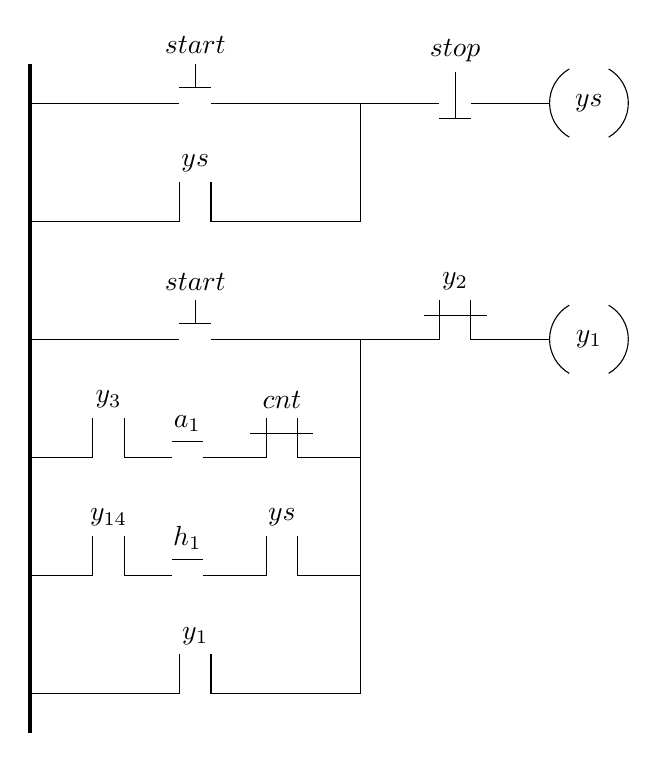
\begin{tikzpicture}[>=triangle 45]
		\draw[ultra thick] (0,0.5) -- (0,-8);
						
		\draw (0,0) -- (1.9,0); \draw (1.9,0.2) -- (2.3, 0.2); \draw (2.1,0.2) -- (2.1, 0.5) node[above]{$start$}; \draw (2.3,0) -- (5.2,0);\draw (5.2,-0.2) -- (5.6,-0.2);  \draw (5.4,-0.2) -- (5.4, 0.4) node[above]{$stop$}; \draw (5.6,0) -- (6.6,0); \draw (6.6,0) arc (180:120:.5);\draw (6.6,0) arc (180:240:.5); \draw (7.6,0) arc (0:60:.5);\draw (7.6,0) arc (0:-60:.5); \draw (7.1,0) node{$ys$}; \draw (0,-1.5) -- (1.9,-1.5) -- (1.9,-1); \draw (2.3,-1) -- (2.3,-1.5) -- (4.2,-1.5) -- (4.2,0); \draw (2.1,-1) node[above]{$ys$};
						
		\draw (0,-3) -- (1.9,-3); \draw (1.9,-2.8) -- (2.3, -2.8); \draw (2.1,-2.8) -- (2.1, -2.5) node[above]{$start$}; \draw (2.3,-3) -- (4.2,-3);
		\draw (0,-4.5) -- (0.8,-4.5) -- (0.8,-4); \draw (1.2,-4) -- (1.2,-4.5) -- (1.8,-4.5); \draw (1,-4) node[above]{$y_3$}; \draw (1.8,-4.3) -- (2.2,-4.3); \draw(2,-4.3) node[above]{$a_1$}; \draw (2.2,-4.5) -- (3,-4.5) -- (3,-4); \draw (3.4,-4) -- (3.4,-4.5) -- (4.2,-4.5); \draw (2.8,-4.2) -- (3.6,-4.2); \draw (3.2,-4) node[above] {$cnt$};
						
		\draw (0,-6) -- (0.8,-6) -- (0.8,-5.5); \draw (1.2,-5.5) -- (1.2,-6)  -- (1.8,-6); \draw (1,-5.5) node[above]{$y_{14}$}; \draw (1.8,-5.8) -- (2.2,-5.8); \draw(2,-5.8) node[above]{$h_{1}$}; \draw (2.2,-6) -- (3,-6) -- (3,-5.5); \draw (3.4,-5.5) -- (3.4,-6) -- (4.2,-6); \draw (3.2,-5.5) node[above] {$ys$};
		\draw (0,-7.5) -- (1.9,-7.5) -- (1.9,-7); \draw (2.3,-7) -- (2.3,-7.5)  -- (4.2,-7.5) -- (4.2,-3); \draw (2.1,-7) node[above]{$y_1$};
						
		\draw (4.2,-3) -- (5.2,-3)-- (5.2,-2.5); \draw (5.6,-2.5) -- (5.6,-3) -- (6.6,-3); \draw (5,-2.7) -- (5.8, -2.7); \draw (5.4,-2.5) node[above]{$y_2$};  \draw (6.6,-3) arc (180:120:.5);\draw (6.6,-3) arc (180:240:.5); \draw (7.6,-3) arc (0:60:.5);\draw (7.6,-3) arc (0:-60:.5); \draw (7.1,-3) node{$y_1$};										
	\end{tikzpicture}
\end{document}